\documentclass[11pt]{article}

% ACL template switch:
% - review: anonymous + line numbers
% - final: camera-ready
% - preprint: non-anonymous with page numbers (depending on template version)
\usepackage[review]{acl}

\usepackage{times}
\usepackage{latexsym}
\usepackage[T1]{fontenc}
\usepackage[utf8]{inputenc}
\usepackage{microtype}
\usepackage{inconsolata}
\usepackage{graphicx}
\usepackage{booktabs}
\usepackage{multirow}
\usepackage{amsmath}
\usepackage{url}

\title{PRDWeaver: Multi-Agent Product Requirements Document Generation with Ablations and Strong-Prompt Baselines}

% For anonymous review, use:
% \author{Anonymous ACL submission}
\author{
  First Author \\
  Affiliation \\
  \texttt{email@domain} \\\And
  Second Author \\
  Affiliation \\
  \texttt{email@domain}
}

\begin{document}
\maketitle

\begin{abstract}
Product Requirements Documents (PRDs) are high-stakes artifacts that bridge user needs, business goals, and implementable technical plans.
We study PRD generation from structured briefs using a modular multi-agent pipeline (\textsc{PRDWeaver}).
We evaluate on a 15-brief benchmark with controlled ablations (e.g., removing alignment, vision, tables, or consistency agents) and compare against several baselines including a strong single-model prompt.
On deliverability-oriented metrics (problem--solution separation and user-journey grounding), the full system significantly outperforms the strong-prompt baseline under Holm--Bonferroni correction, while a targeted ablation (\texttt{no\_table}) predictably eliminates tables.
\end{abstract}

\section{Introduction}
\label{sec:intro}

Product Requirements Documents (PRDs) are high-stakes planning artifacts that connect user needs, business objectives, and implementable technical requirements.
In practice, teams rely on PRDs to align stakeholders, define scope, and reduce downstream rework; however, producing high-quality PRDs is time-consuming and error-prone.
Recent large language models (LLMs) can draft long-form documents, but maintaining \emph{executability} (clear requirements), \emph{grounded user reasoning} (personas and journeys), and \emph{consistent structure} remains challenging for single-pass generation.

We study PRD generation from structured product briefs using a modular multi-agent pipeline, \textsc{PRDWeaver}.
Rather than relying on a single monolithic prompt, \textsc{PRDWeaver} composes specialized agents (e.g., alignment, table, and consistency agents) orchestrated by a pipeline controller, and an assembler that produces a schema-conformant PRD.
This modularity enables controlled ablations that test which components contribute to document quality.

We evaluate on a benchmark of 15 diverse briefs and compare against multiple baselines, including a strong single-model prompting baseline (\textsc{StrongPrompt}) designed to explicitly request key PRD sections.
Our analysis uses paired nonparametric tests (Wilcoxon signed-rank) with Holm--Bonferroni correction and effect sizes (Cliff's delta).

\paragraph{Contributions.}
We contribute:
(i) a modular multi-agent PRD generation pipeline with an \emph{ablation-safe} design (no-op agents preserve message flow so all variants remain comparable),
(ii) a reproducible benchmark and automated PRD quality evaluation suite with multiple-comparison corrected statistics,
and (iii) a practical artifact package: a Web API and an optional MCP tool interface for generation and metric-based evaluation.

\section{Task and Benchmark}
\label{sec:task}

\paragraph{Input.}
Each instance is a structured product brief describing a product context, target users, goals, and constraints.

\paragraph{Output.}
The system produces a PRD in a fixed schema with sections such as overview, personas, user stories, user flows, functional and non-functional requirements, key interfaces, KPIs and milestones, risks and mitigations, data/tracking, and release plan.

\paragraph{Benchmark.}
We evaluate on 15 briefs spanning domains such as ecommerce, education, finance, healthcare, and general productivity.
All systems are run on the same set of briefs, producing paired samples for statistical comparison.

\section{System: \textsc{PRDWeaver}}
\label{sec:system}

\textsc{PRDWeaver} is a modular, multi-agent pipeline that generates a schema-conformant PRD from a brief.
The orchestrator routes intermediate artifacts between agents, and a final assembler produces the output PRD.

\begin{figure}[t]
  \centering
  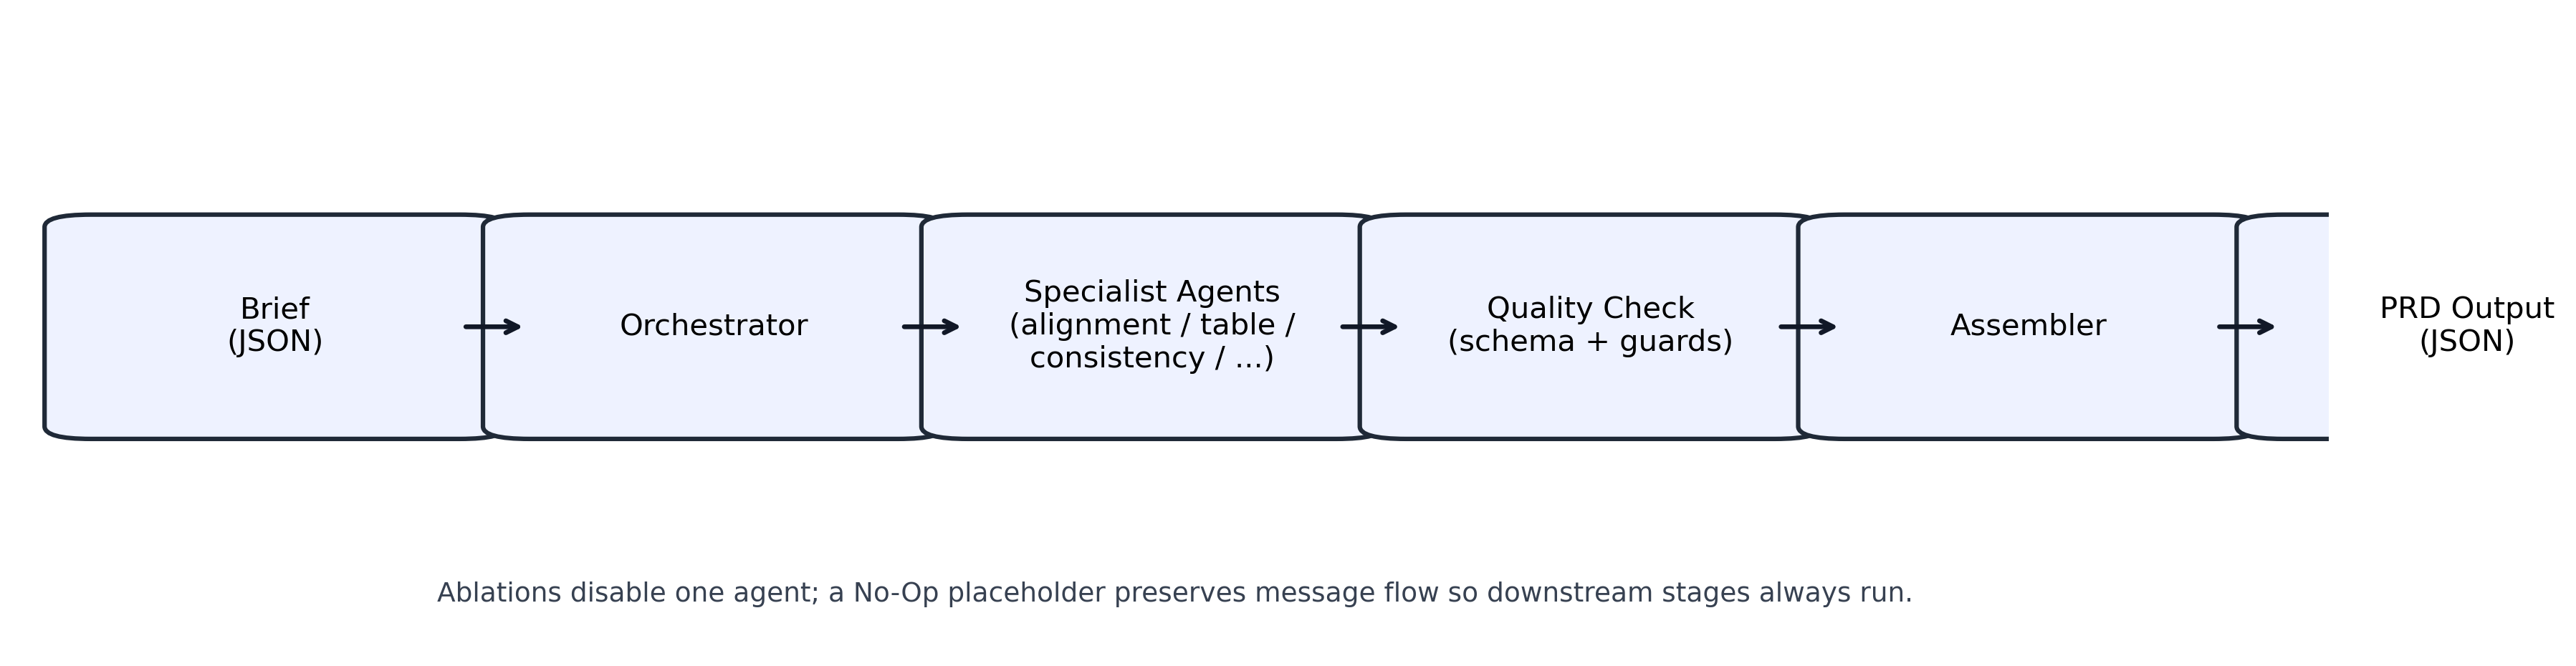
\includegraphics[width=\columnwidth]{figures/framework_pipeline.png}
  \caption{System overview. \textsc{PRDWeaver} orchestrates specialist agents and assembles a schema-conformant PRD. In ablations, disabled agents are replaced by a no-op placeholder to preserve message flow.}
  \label{fig:framework}
\end{figure}

\paragraph{Agents.}
We use specialized agents for complementary roles, including:
(i) an alignment agent to restate goals and constraints,
(ii) an optional table agent to structure content into tables when applicable,
(iii) a consistency agent to enforce terminology and section-to-section coherence,
and (iv) a quality/verification stage that validates schema completeness prior to assembly.

\paragraph{Ablation-ready design.}
To enable controlled ablations, disabled agents are replaced with a no-op placeholder that preserves message flow.
This prevents pipeline breaks and ensures that downstream stages (quality checks and assembly) always run, making ablation outputs directly comparable.

\section{Automatic Metrics}
\label{sec:metrics}

We report a set of automated metrics that capture PRD structure and quality dimensions.
Some metrics are binary/structural (e.g., presence of required sections, tables), while others approximate semantic quality (e.g., problem clarity, requirement executability, terminology consistency) via rubric-based checks.

\paragraph{Statistical testing.}
All comparisons use paired samples across the same 15 briefs.
We apply the Wilcoxon signed-rank test and report effect sizes using Cliff's delta.
To control family-wise error across multiple metrics, we apply Holm--Bonferroni correction and report corrected \(q\)-values.

\section{Experiments}
\label{sec:experiments}

We evaluate the full system, ablation variants (e.g., \texttt{no\_alignment}, \texttt{no\_vision}, \texttt{no\_table}, \texttt{no\_consistency}), and baselines including a strong single-model prompt (\textsc{StrongPrompt}).
Each system produces PRDs for all 15 briefs; we compute paired metrics and perform corrected significance testing.

\paragraph{Reproducibility and artifacts.}
We provide a CLI and a Web API to reproduce generations and compute metrics on arbitrary PRDs.
The Web API supports controlled configurations (e.g., disabling agents and selecting a model provider), enabling standardized evaluation without manual annotation.

\section{Results}
\label{sec:results}

\subsection{Ablation Study}
Removing the table agent (\texttt{no\_table}) eliminates tables as designed, with \(S_{\mathrm{tab}}\) dropping from 1.0 to 0.0 (corrected \(q<0.01\)), validating that the ablation controls the targeted capability.

% Auto-generated by scripts/export_paper_assets.py
\begin{table*}[t]
\centering
\small
\setlength{\tabcolsep}{4pt}
\begin{tabular}{lrrrrrr}
\toprule
Metric & Full & no\_table & no\_consistency & no\_alignment & no\_vision & async\_queue \\
\midrule
S\_sem & 0.8805 & 0.8805 & 0.8778 & 0.8805 & 0.8750 & 0.8805 \\
S\_ps & 1.0000 & 1.0000 & 1.0000 & 1.0000 & 1.0000 & 1.0000 \\
S\_uj & 1.0000 & 0.9778 & 0.9778 & 0.9704 & 0.9778 & 1.0000 \\
S\_hyp & 1.0000 & 1.0000 & 1.0000 & 1.0000 & 1.0000 & 1.0000 \\
S\_tab & 1.0000 & \textbf{0.0000} & 1.0000 & 0.9333 & 0.9333 & 1.0000 \\
S\_bi & 0.5074 & 0.5631 & 0.5639 & 0.5636 & 0.5615 & 0.5583 \\
\bottomrule
\end{tabular}
\caption{Ablation summary (means over 15 briefs). Removing the Table agent (\texttt{no\_table}) eliminates tables by design (bold).}
\label{tab:ablation-summary}
\end{table*}


\subsection{Full System vs. StrongPrompt Baseline}
The full system significantly improves deliverability-oriented metrics over \textsc{StrongPrompt} after correction:
\(S_{\mathrm{ps}}\) (\(\Delta=+0.6811\), \(q=0.0060\)),
\(S_{\mathrm{uj}}\) (\(\Delta=+0.6389\), \(q=0.0066\)),
and \(S_{\mathrm{hyp}}\) (\(\Delta=+0.6000\), \(q=0.0066\)).
We observe a trade-off on bilingual compliance \(S_{\mathrm{bi}}\), where \textsc{StrongPrompt} scores higher (\(\Delta=-0.0672\), \(q=0.0013\)).

% Auto-generated by scripts/export_paper_assets.py
\begin{table}[t]
\centering
\small
\setlength{\tabcolsep}{4pt}
\begin{tabular}{lrrrr}
\toprule
Metric & Full & StrongPrompt & $\Delta$ & $q$ \\
\midrule
S\_sem & 0.8805 & 0.7722 & 0.1083 & 0.0639 \\
S\_ps & 1.0000 & 0.3189 & 0.6811 & \textbf{0.0060} \\
S\_uj & 1.0000 & 0.3611 & 0.6389 & \textbf{0.0066} \\
S\_hyp & 1.0000 & 0.4000 & 0.6000 & \textbf{0.0066} \\
S\_bi & 0.5597 & 0.6269 & -0.0672 & \textbf{0.0013} \\
S\_tab & 1.0000 & 1.0000 & 0.0000 & 1.0000 \\
S\_biz & 0.5000 & 0.5111 & -0.0111 & 1.0000 \\
S\_tech & 1.0000 & 1.0000 & 0.0000 & 1.0000 \\
S\_risk & 1.0000 & 1.0000 & 0.0000 & 1.0000 \\
S\_comp & 1.0000 & 1.0000 & 0.0000 & 1.0000 \\
S\_mm & 1.0000 & 1.0000 & 0.0000 & 1.0000 \\
S\_expert & 1.0000 & 1.0000 & 0.0000 & 1.0000 \\
S\_var & 0.0000 & 0.0000 & 0.0000 & 1.0000 \\
\bottomrule
\end{tabular}
\caption{Full system vs. StrongPrompt baseline on 15 briefs. $\Delta$ = Full $-$ StrongPrompt. $q$ is Holm--Bonferroni corrected Wilcoxon p-value.}
\label{tab:full-vs-strong}
\end{table}


\begin{figure}[t]
  \centering
  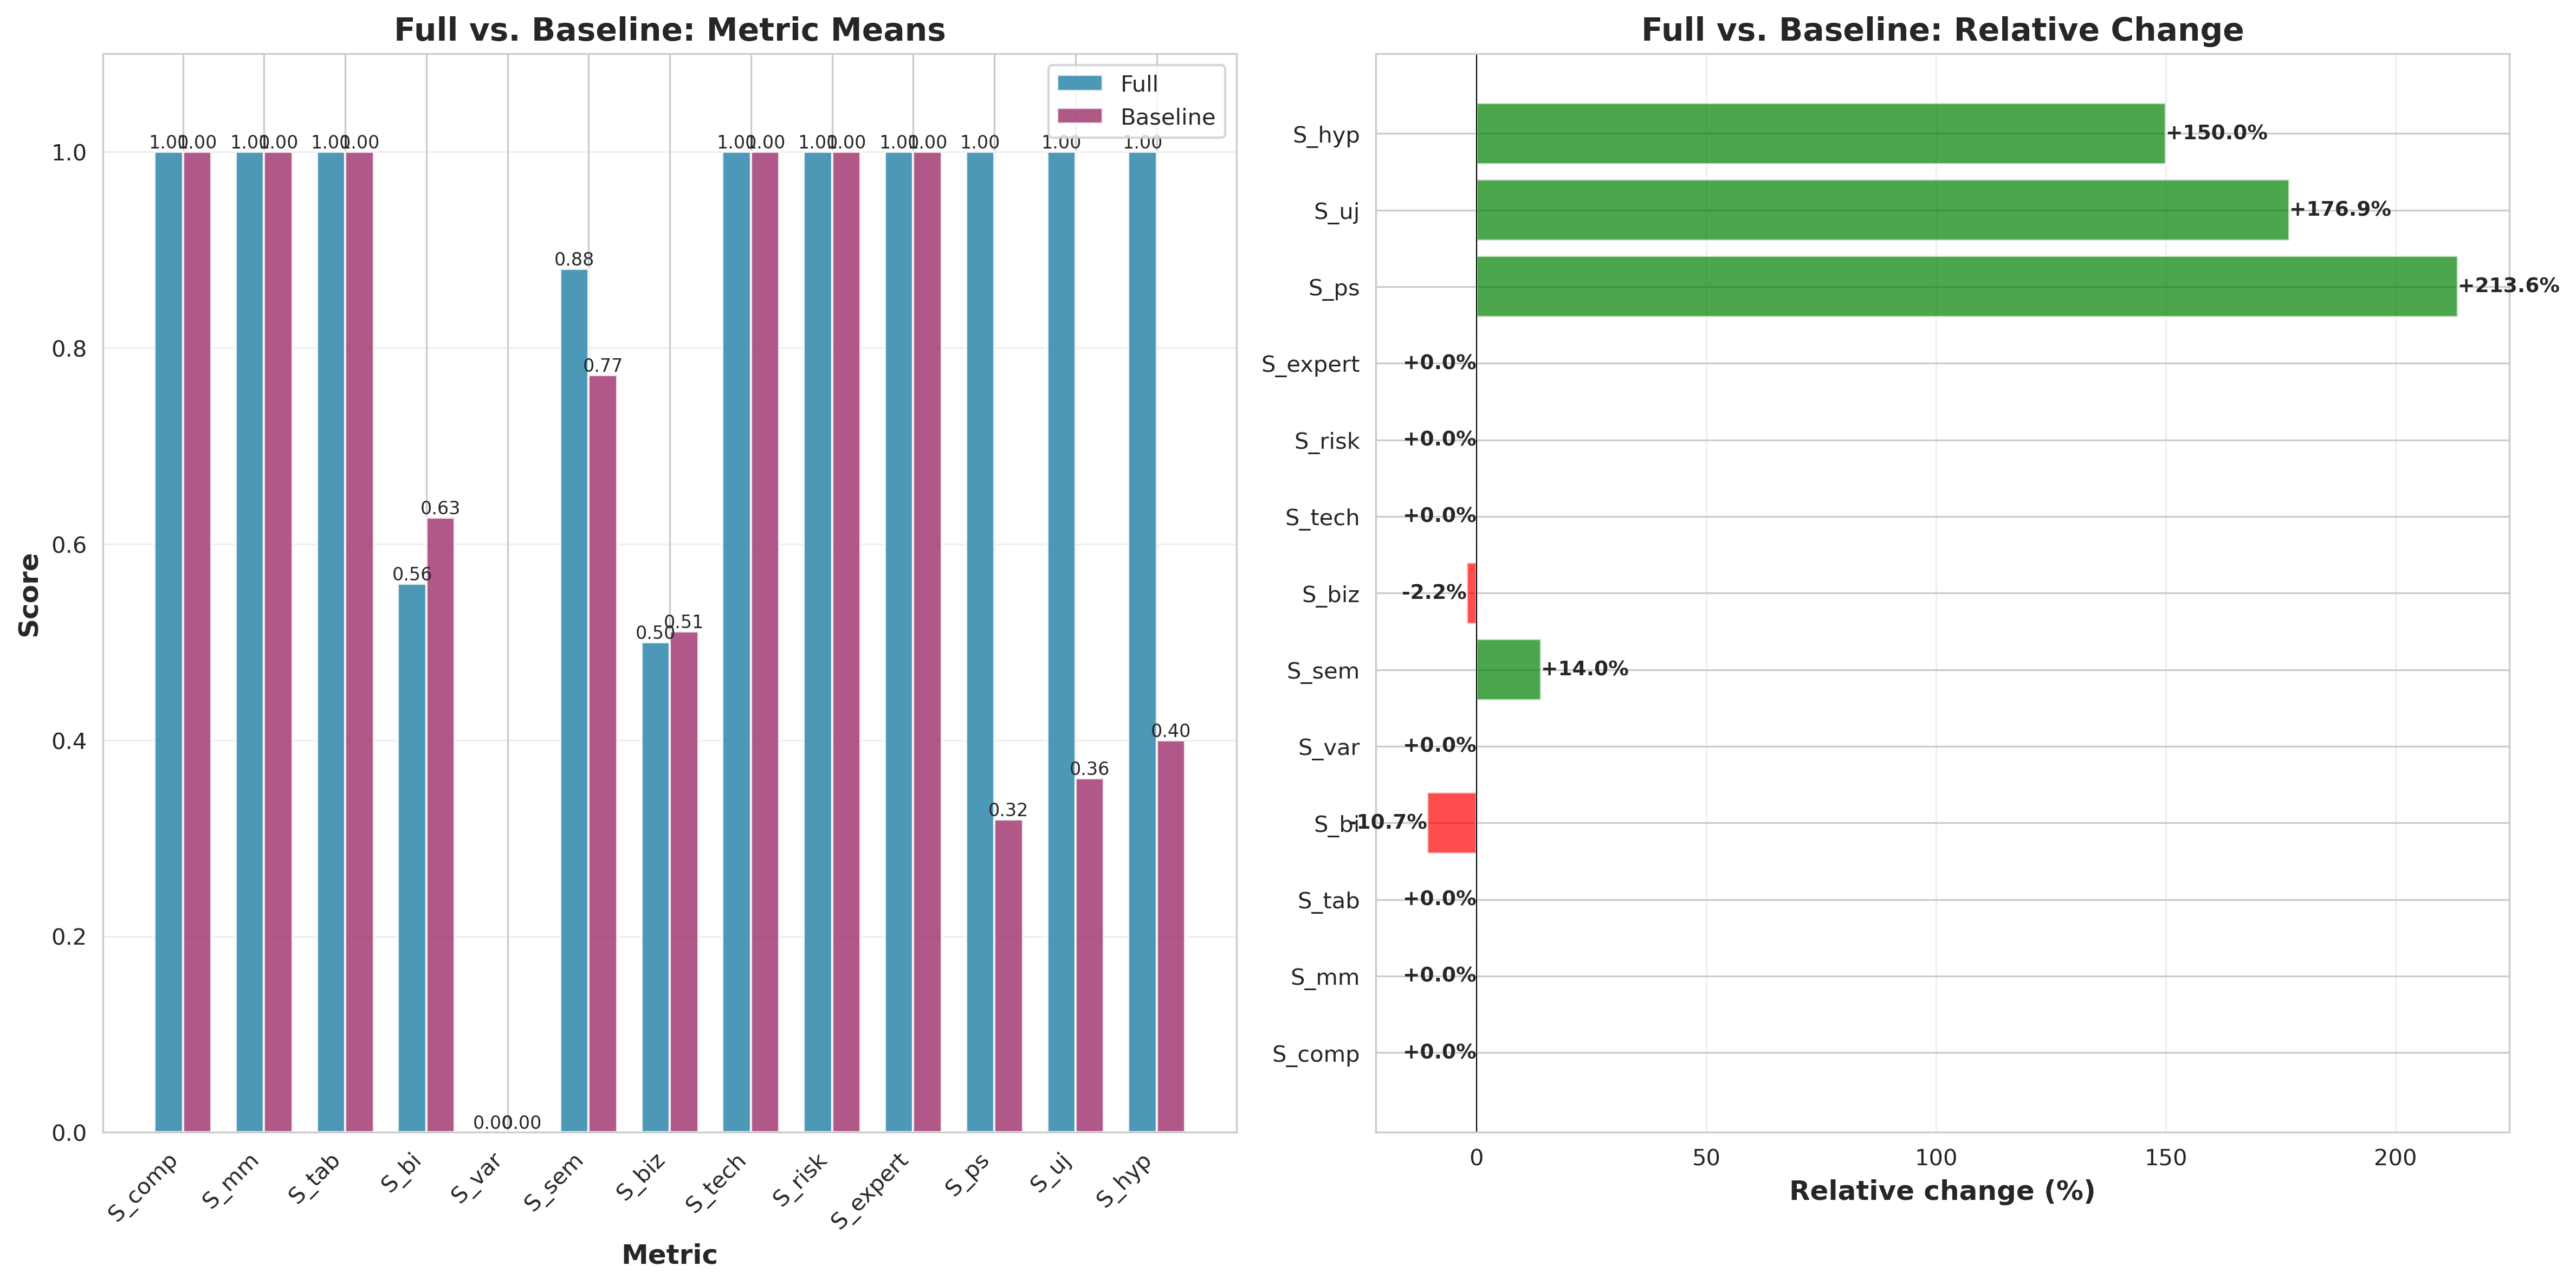
\includegraphics[width=\columnwidth]{figures/full_vs_strong_prompt_comparison.png}
  \caption{Full system vs. StrongPrompt baseline across metrics (means over 15 briefs).}
  \label{fig:full-strong}
\end{figure}

\begin{figure}[t]
  \centering
  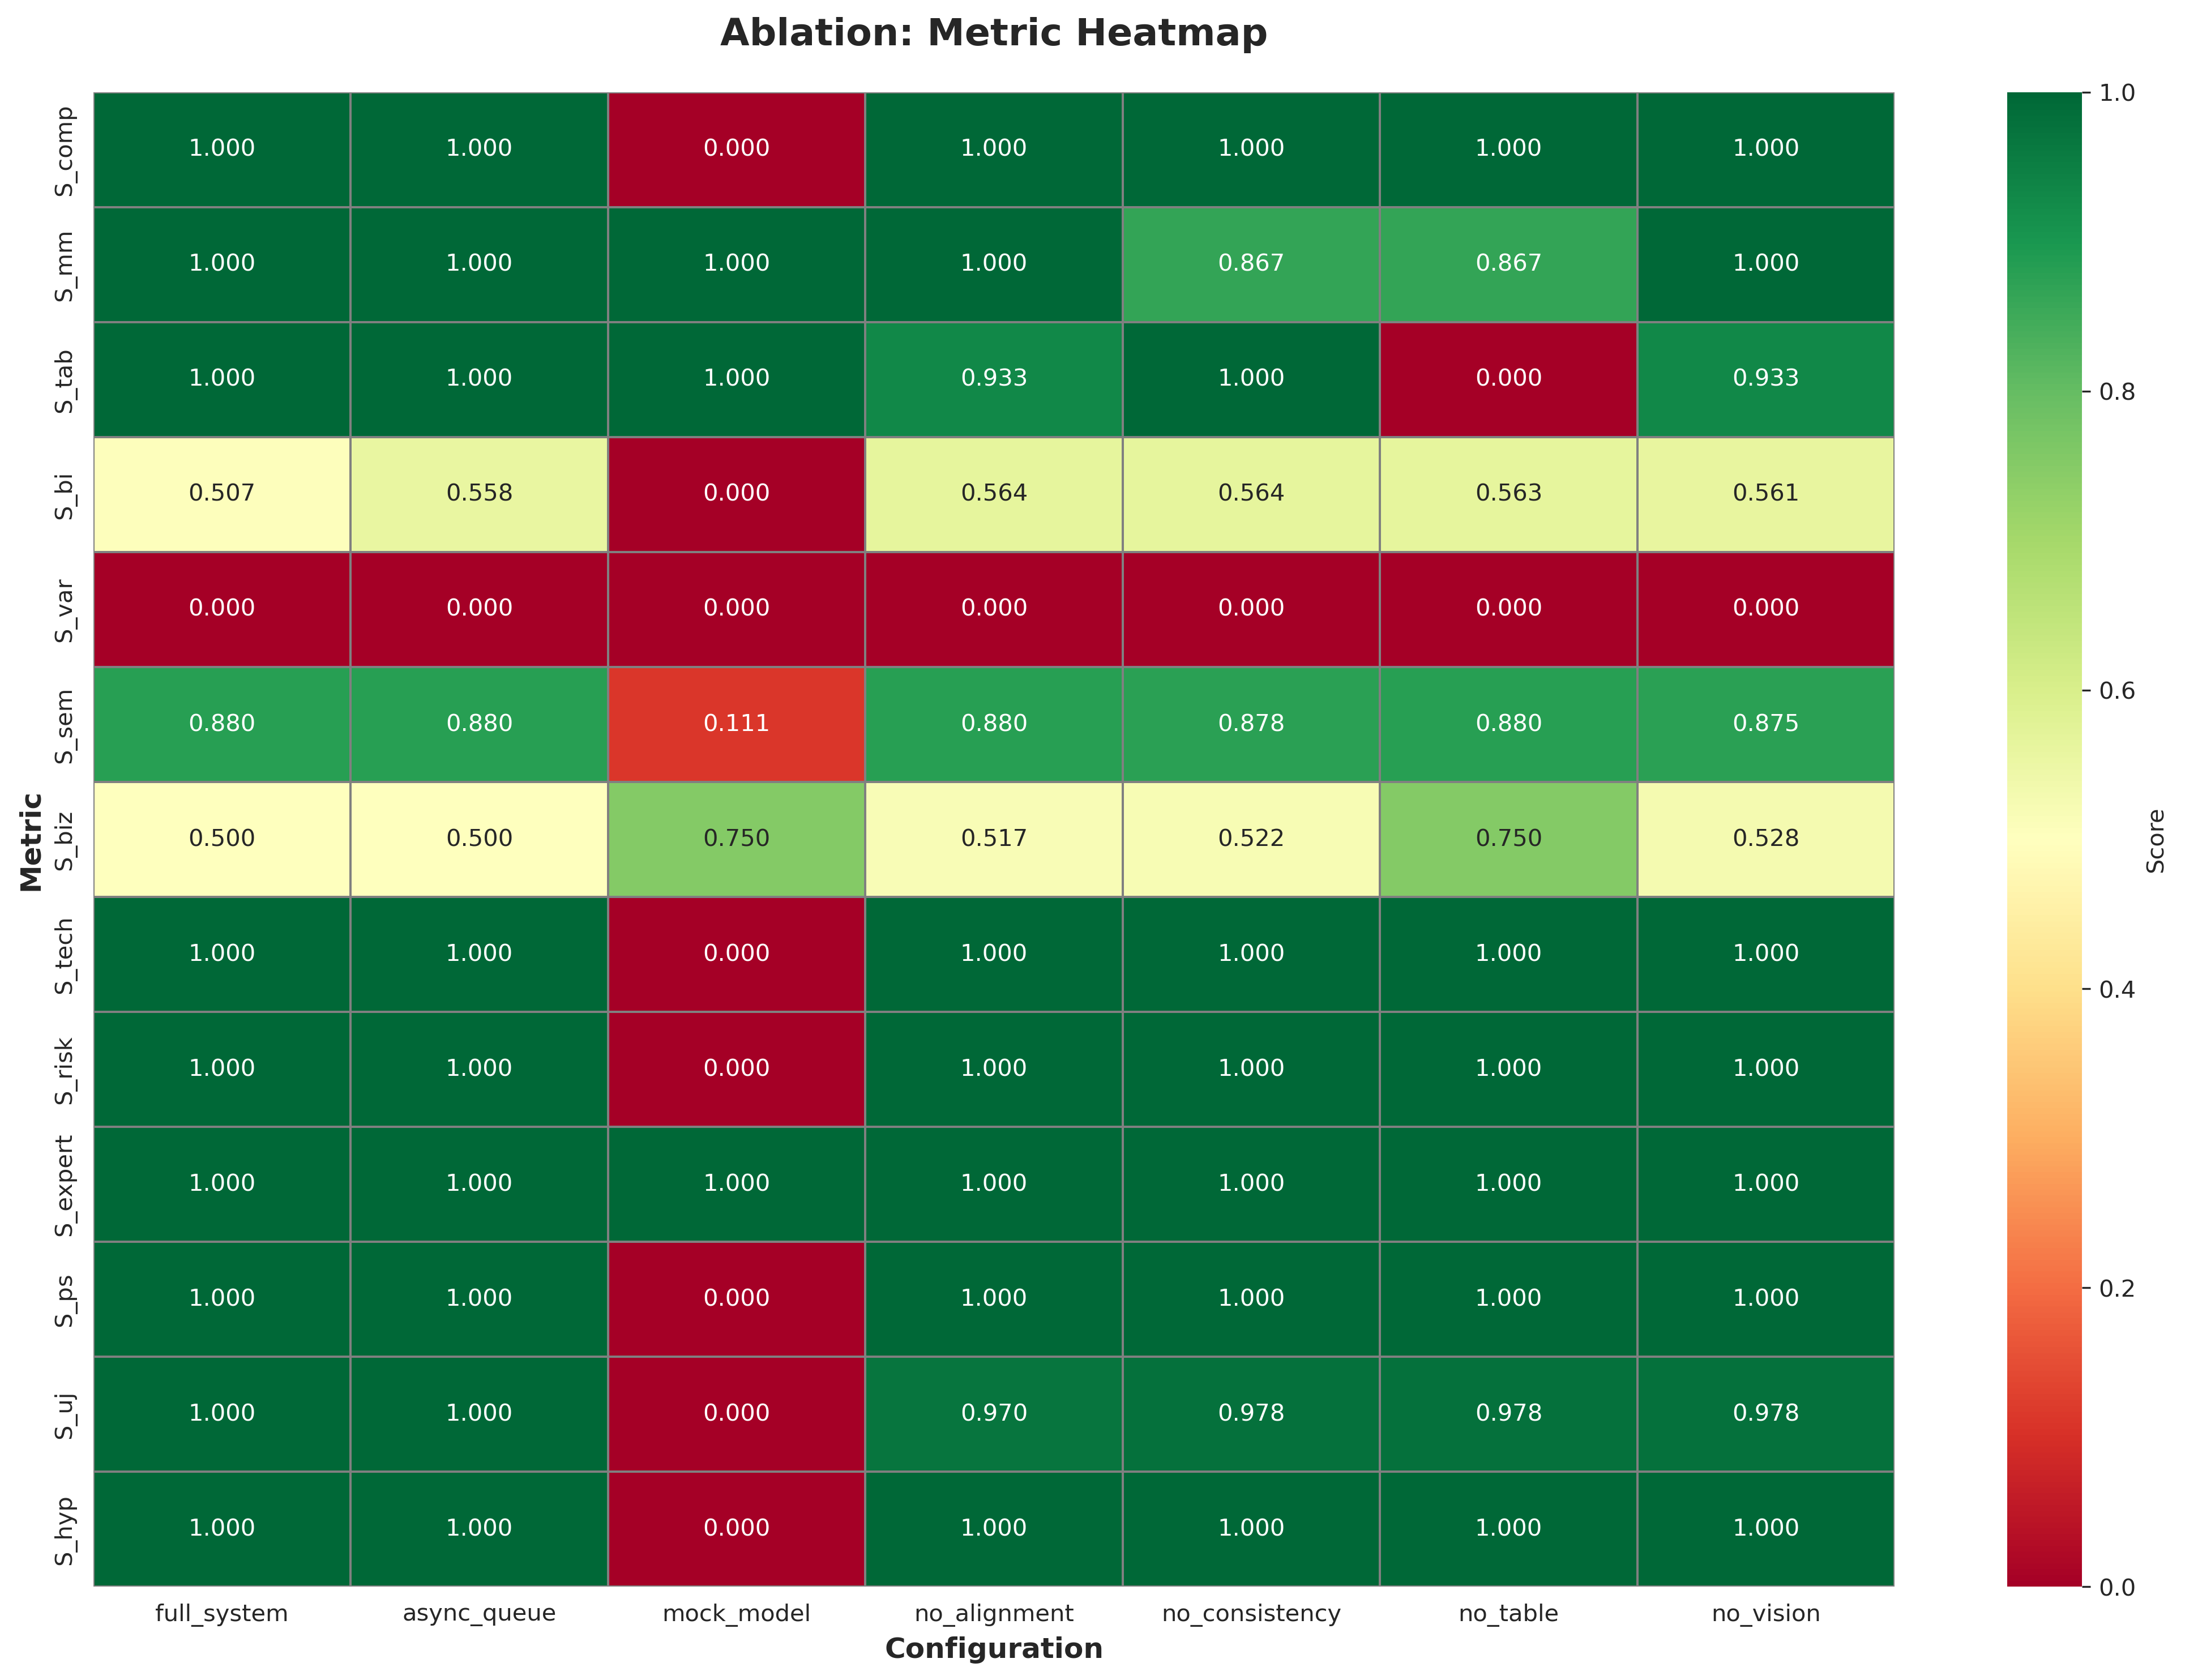
\includegraphics[width=\columnwidth]{figures/ablation_heatmap.png}
  \caption{Ablation heatmap: mean metric values per configuration (15 briefs).}
  \label{fig:ablation-heatmap}
\end{figure}

\section*{Limitations}
Our evaluation relies heavily on automated metrics, some of which are structural and may saturate when systems reliably emit required sections.
Semantic quality proxies are imperfect and do not fully replace expert human judgment.

\paragraph{Why some gains look ``large''.}
Several headline improvements (e.g., problem--solution separation and user-journey grounding) are measured as rubric-style compliance scores.
When a baseline frequently omits these artifacts, the metric can change sharply once a system reliably produces them.
We therefore prioritize comparisons against \textsc{StrongPrompt} and report multiple-comparison corrected significance.

\section*{Ethics Statement}
Generated PRDs may contain errors or hallucinations and should be reviewed by humans before use in real decision-making.

\section{Conclusion}
\label{sec:conclusion}
We presented \textsc{PRDWeaver}, a modular multi-agent PRD generation pipeline, and evaluated it under controlled ablations and strong baselines.
On a 15-brief benchmark, the full system significantly improves deliverability-oriented dimensions over a strong prompting baseline.

\bibliographystyle{acl_natbib}
\bibliography{custom}

\end{document}


